\documentclass[aspectratio=169]{beamer}
\setbeamertemplate{navigation symbols}{}
\usepackage{color,amsmath,comment, subfigure}
\usepackage{booktabs}
\usepackage{url}

%%%%%%%%%%%%%%%%%%%%%%%%%%
\title[]{Lecture 22: Network scale-up method to study groups most at-risk for HIV}
\author[]{Matthew J. Salganik}
\institute[]{Sociology 204: Social Networks\\Princeton University}
\date[]{
Pre-read
\vfill

\begin{flushleft}
\vspace{0.6in}

\includegraphics[width=0.1\textwidth]{figures/cc.png}
\end{flushleft}
}

\begin{document}
%%%%%%%%%%%%%%%%%%%%%%%%%%%
\frame{\titlepage}
%%%%%%%%%%%%%%%%%%%%%%%%%%%
\begin{frame}

There are an estimated 38 million people [31.6 million–44.5 million] living with HIV in 2019.  In most countries, the disease is concentrated in three high risk groups:
\begin{itemize}
\item drug users 
\item commercial sex workers
\item men who have sex with men 
\end{itemize}
\vfill
Better information about these group can be used to understand and control the spread of HIV/AIDS: ``know your epidemic''
\end{frame}
%%%%%%%%%%%%%%%%%%%%%%%%%
\begin{frame}

Two main questions:
\begin{itemize}
\item prevalence of some trait within a hidden population (e.g., What proportion of sex workers in Moscow have HIV/AIDS?): \pause respondent-driven sampling (lecture 13) \pause
\item size of hidden population (e.g., How many sex workers are there in Moscow?) \pause network scale-up method (this lecture)
\end{itemize}

\end{frame}
%%%%%%%%%%%%%%%%%%%%%%%%%
\begin{frame}

\LARGE{Network scale-up method}

\end{frame}
%%%%%%%%%%%%%%%%%%%%%%%%
\begin{frame}
\frametitle{}

\begin{center}
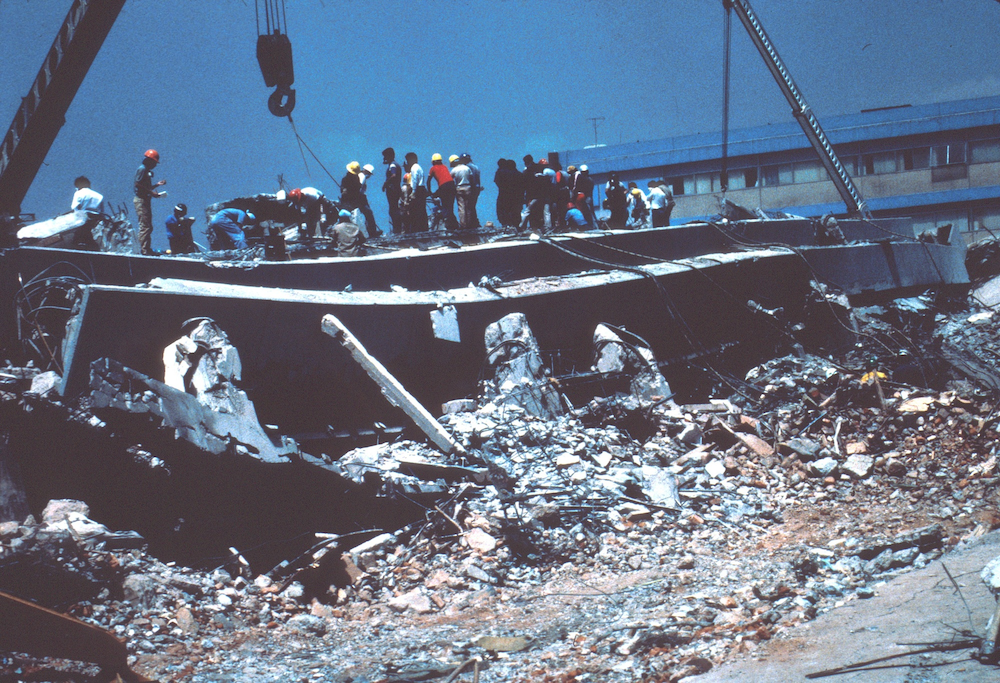
\includegraphics[width=0.8\textwidth]{figures/1985_Mexico_Earthquake_smaller.png}
\end{center}

Basic insight from Bernard et al. (1989)

\end{frame}
%%%%%%%%%%%%%%%%%
\begin{frame}

\begin{center}
\includegraphics<1>[width=0.6\textwidth]{figures/network-noedges}
\includegraphics<2>[width=0.6\textwidth]{figures/network-edges}
\includegraphics<3>[width=0.6\textwidth]{figures/network-edges-sample}
\includegraphics<4>[width=0.6\textwidth]{figures/network-edges-sample-ego}
\end{center}
\Large{
\begin{center}
\onslide<4>{$\hat{N}_H=\frac{2}{10} \times 30 = 6$}
\end{center}
}

\end{frame}
%%%%%%%%%%%%%%%%%
\begin{frame}

\begin{itemize}
\item Requires a random sample from the entire population 
\item Respondents are asked:
\begin{itemize}
\item How many people do you know who are drug injectors? 
\item How many women do you know that have given birth in the last 12 months?
\item How many people do you know who are middle school teachers?
\item $\ldots$
\item How many people do you know named Michael?
\end{itemize}
\item ``Know'' typically defined: you know them and they know you and have you been in contact with them over the past two years
\end{itemize}

\end{frame}
%%%%%%%%%%%%%%%%%
\begin{frame}

\begin{center}
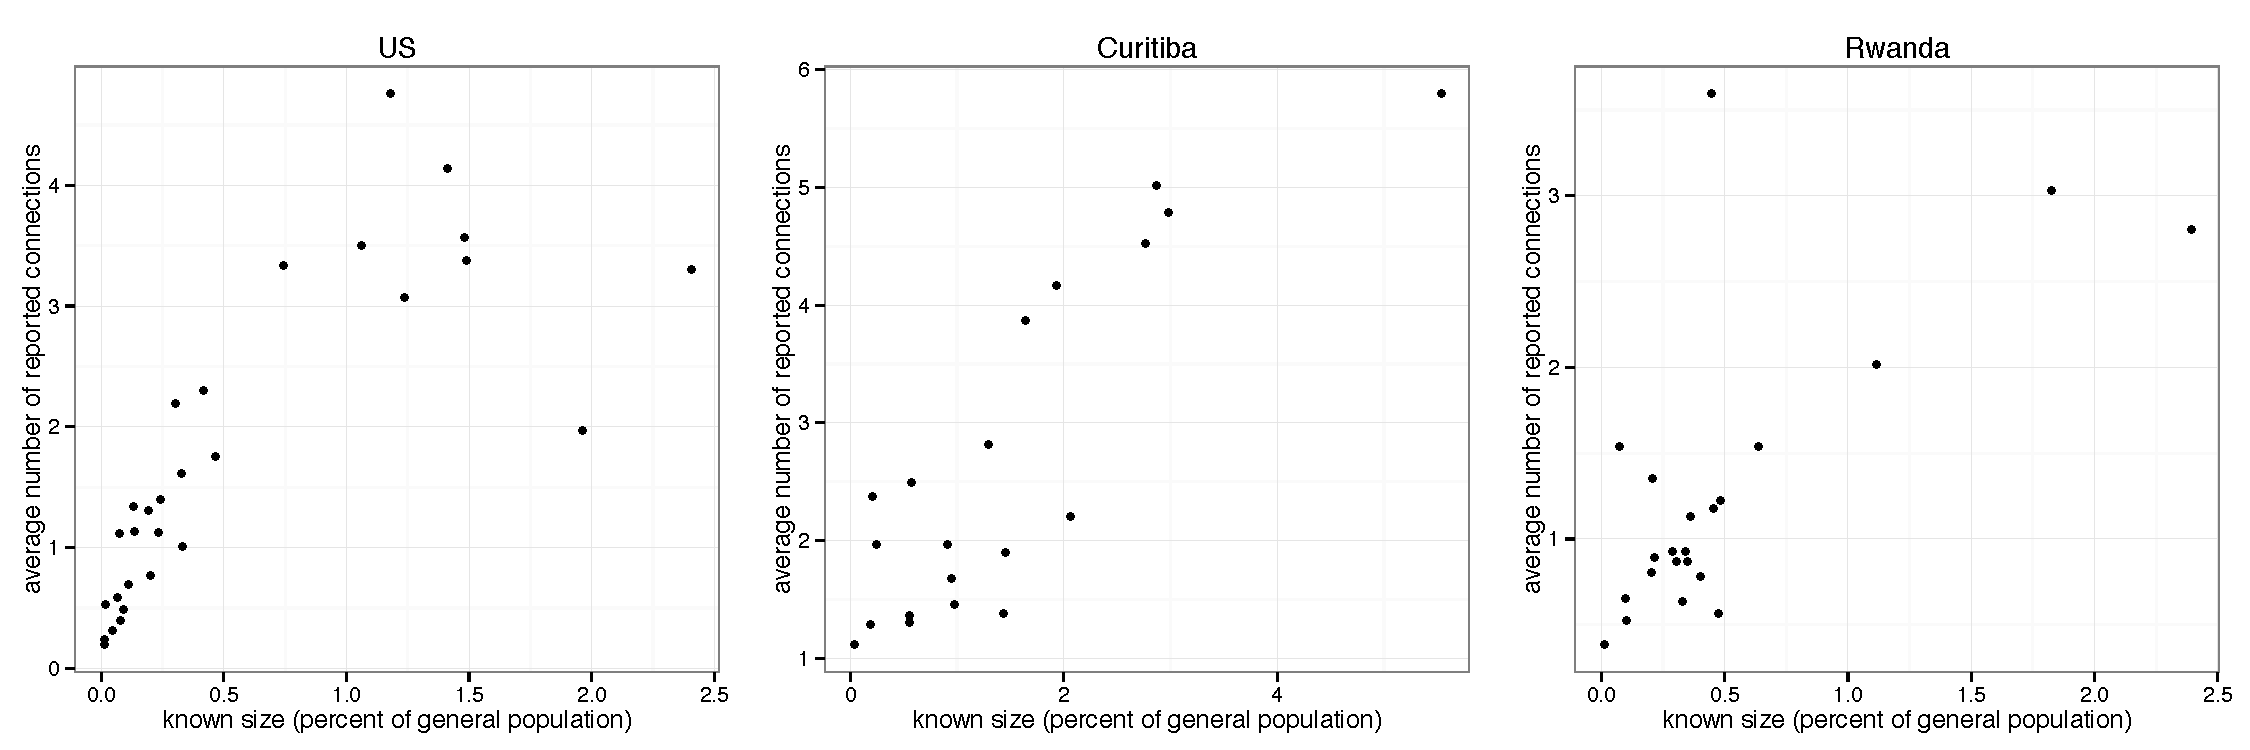
\includegraphics[width=0.95\textwidth]{figures/three_studies_truesize_known}
\end{center}
\vfill
On average, these answers are not crazy.

\end{frame}
%%%%%%%%%%%%%%%%%%
\begin{frame}

Other size estimation methods are problematic, and scale-up method has many nice properties:
\begin{itemize}
\item Requires a random sample of the general population, not specific contact with the hard-to-reach population \pause
\item Can be added as a module (5-10 minutes) in any existing survey \pause
\item Can estimate many target populations in a single survey \pause
\item Can be applied at the city-level, sub-national-level, or national-level \pause
\item Statistical methods are improvable \pause
\item Partially self-validating because it uses groups of known size
\end{itemize}

\end{frame}
%%%%%%%%%%%%%%%%%
\begin{frame}

\begin{figure}
  \centering
   \subfigure[United States]{
     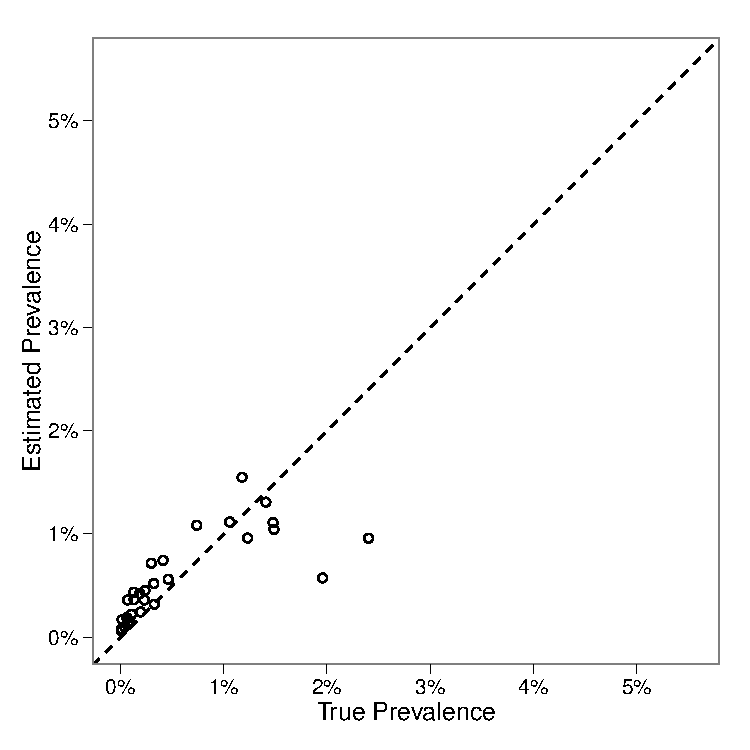
\includegraphics[width=0.3\textwidth]{figures/us-ivplot-forr01}}
  \hspace{0.0in}
    \subfigure[Curitiba]{
     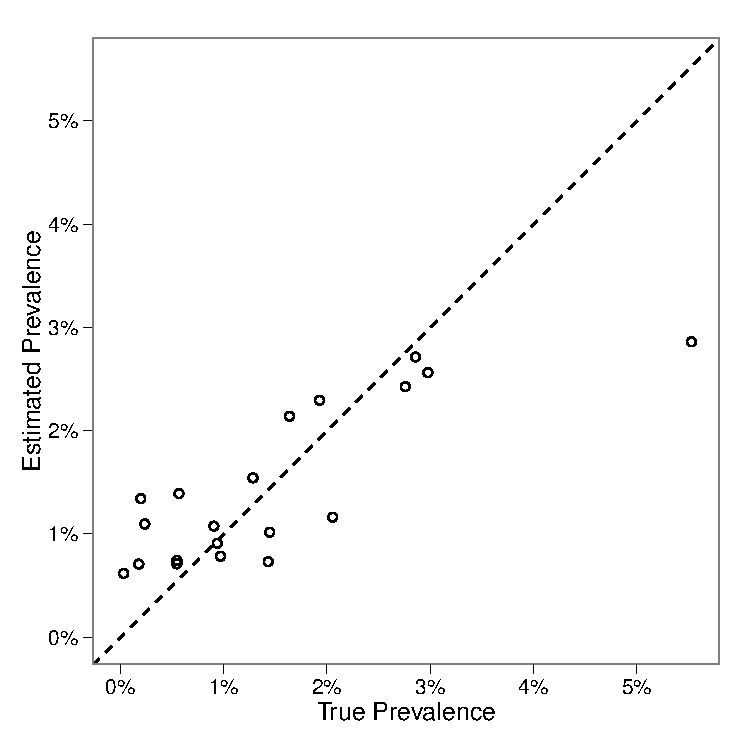
\includegraphics[width=0.3\textwidth]{figures/curitiba-ivplot-forr01}}     
  \hspace{0.0in}
    \subfigure[Rwanda]{
     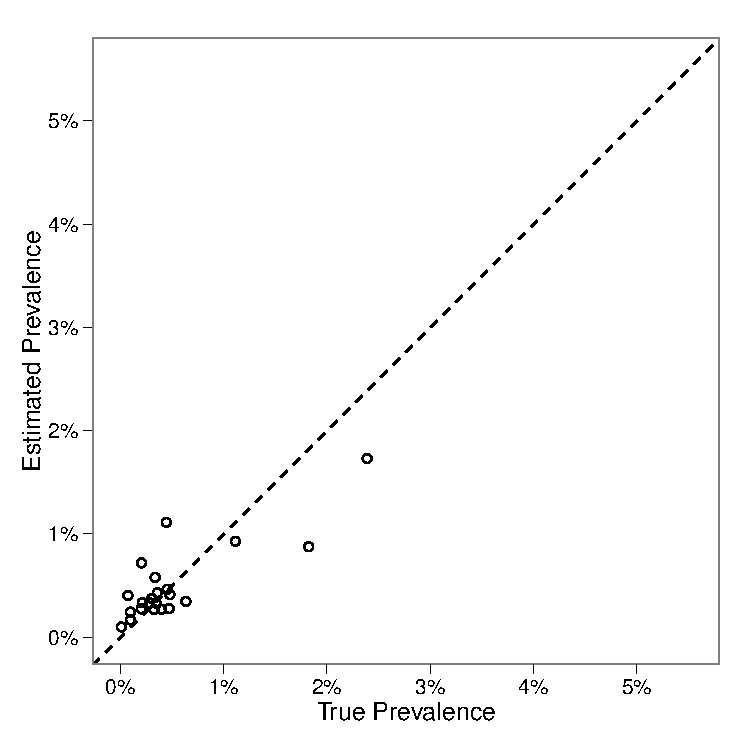
\includegraphics[width=0.3\textwidth]{figures/rwanda-ivplot-forr01}}     
\end{figure}

\end{frame}
%%%%%%%%%%%%%%%%
\begin{frame}

\LARGE{Network scale-up method, basic estimator}

\end{frame}
%%%%%%%%%%%%%%%%%%%%%%%%
\begin{frame}

\begin{equation*}
\hat{N}_H = \frac{\sum_i y_{i,H}}{\sum_i \hat{d}_i} \times N
\end{equation*}
\small{
\begin{itemize}
\item $\hat{N}_H$: number of people in the hidden population
\item $y_{i,H}$: number of people in hidden population known by person $i$
\item $\hat{d}_i$: estimated number of people known by person $i$
\item $N$: number of people in the population
\end{itemize}
}

\end{frame}
%%%%%%%%%%%%%%%%%
\begin{frame}

\begin{equation*}
\hat{d}_i =  \frac{\sum_k y_{i,k}}{\sum_k N_k} \times N
\end{equation*}
\small{
\begin{itemize}
\item $\hat{d}_i$: estimated number of people known by person $i$
\item $y_{i,k}$: number of people in group $k$ known by person $i$
\item $N_k$: number of people in group $k$
\item $N$: number of people in the population
\end{itemize}
}

\end{frame}
%%%%%%%%%%%%%%%%%
\begin{frame}

\begin{equation*}
\hat{d}_i = \frac{\sum_k y_{i,k}}{\sum_k N_k} \times N
\end{equation*}
\small{
\begin{itemize}
\item $\hat{d}_i$: estimated number of people known by person $i$
\item $y_{i,k}$: number of people in group $k$ known by person $i$
\item $N_k$: number of people in group $k$
\item $N$: number of people in the population
\end{itemize}
}

There are 50,000 Nsabimanas in Rwanda and 10 million people in Rwanda.  You know 2 Nsabimanas.  We estimate you know:
\pause
\begin{equation*}
\hat{d}_i = \frac{2}{50,000} \times 10 \mbox{ million} = 400 \mbox{ people} 
\end{equation*}

\end{frame}
%%%%%%%%%%%%%%%%
\begin{frame}

\begin{equation*}
\hat{d}_i = \frac{\sum_k  y_{i,k}}{\sum_k N_k} \times N
\end{equation*}
\small{
\begin{itemize}
\item $\hat{d}_i$: estimated number of people known by person $i$
\item $y_{i,k}$: number of people in group $k$ known by person $i$
\item $N_k$: number of people in group $k$
\item $N$: number of people in the population
\end{itemize}
}

There are 50,000 Nsabimanas in Rwanda; 1,000 Priests; and 10 million people in Rwanda.  You know 2 Nsabimanas and 1 priest.  We estimate you know:
\pause
\begin{equation*}
\hat{d}_i = \frac{2 + 1}{50,000 + 1,000} \times 10 \mbox{ million} \approx 600 \mbox{ people} 
\end{equation*}

\end{frame}
%%%%%%%%%%%%%%%%%%%%%%%%%%%%%%%%
\begin{frame}

\begin{equation*}
\hat{N}_H = \frac{\sum_i y_{i,H}}{\sum_i \hat{d}_i} \times N
\end{equation*}
\small{
\begin{itemize}
\item $\hat{N}_H$: number of people in the hidden population
\item $y_{i,H}$: number of people in hidden population known by person $i$
\item $\hat{d}_i$: estimated number of people known by person $i$
\item $N$: number of people in the population
\end{itemize}
}

\begin{itemize}
\item Person 1 knows 2 female sex workers and 400 people
\item Person 2 knows 4 female sex workers and 600 people
\end{itemize}
\pause
\begin{equation*}
\hat{N}_H  = \frac{2 + 4}{400 + 600} \times 10 \mbox{ million} = 60,000 \mbox{ people} 
\end{equation*}

\end{frame}
%%%%%%%%%%%%%%%%%
\begin{frame}

\begin{center}
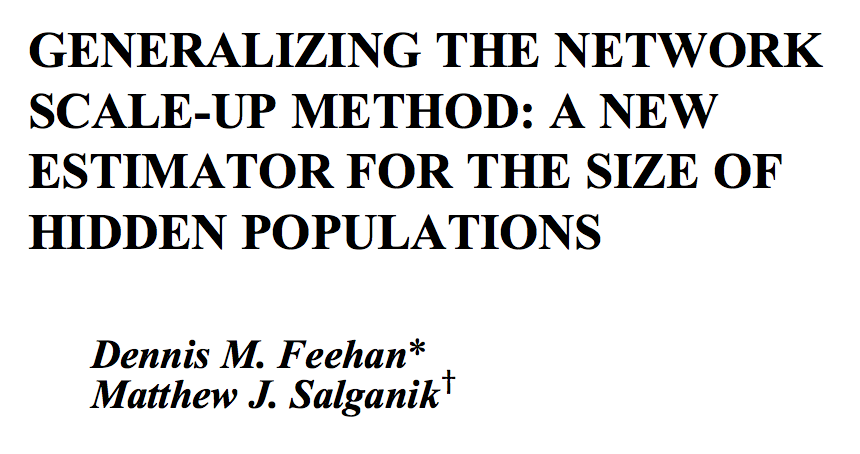
\includegraphics[width=0.5\textwidth]{figures/feehan_generalizing_2016_title}
\end{center}

\begin{itemize}
\item We develop the generalized scale-up estimator and use it to point out possible biases in basic scale-up estimator, but requires two data collections, which is rare (but wait until lecture 23) \pause
\item For the purposes of this class, focus on basic scale-up estimator and the correction factors needed for it
\end{itemize}

\end{frame}
%%%%%%%%%%%%%%%%%%%%%%%%%%%%%%%%%
\begin{frame}

\begin{center}

\includegraphics[width=0.5\textwidth]{figures/feehan_quantity_2016_title}
\end{center}

\begin{itemize}
\item Are there tie definitions other than ``to know'' that would lead to better estimates? We did a survey experiment to compare different definitions and then combined them to produce a single estimate \pause
\item Notice how we decided which is better and how we combined estimates \pause
\item Notice how we dealt with the many things we did not know with sensitivity analysis. 
\end{itemize}

\end{frame}
%%%%%%%%%%%%%%%%%%%%%%%%%
\begin{frame}

{\Large
\begin{center}
Enjoy the reading
\end{center}
}

\end{frame}

\end{document}
